\documentclass[../../main.tex]{subfiles}
\begin{document}

$xy$ 平面において，点 $A$ は原点 $O$ を中心とする半径1の円周の第1象限にある部分を動き，点 $B$ は $x$ 軸上を動く．
ただし，線分 $AB$ の長さは1であり，線分 $AB$ は両端 $A$，$B$ 以外の点 $C$ で円周と交わるものとする．

\begin{figure}[htbp]
  \centering
  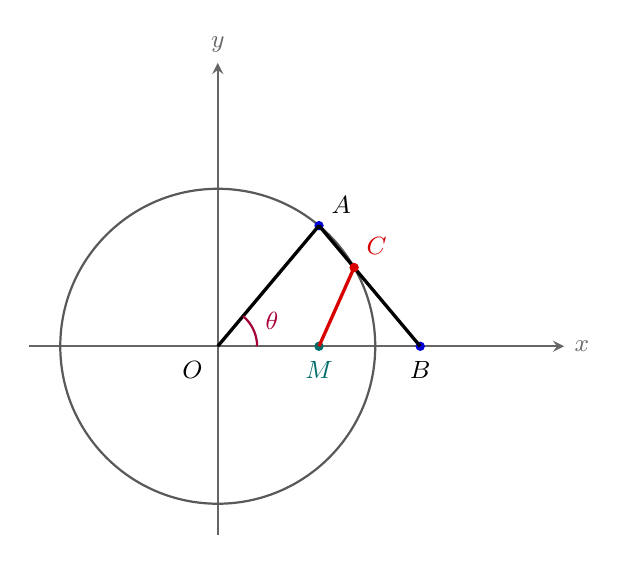
\begin{tikzpicture}[scale=2, >=stealth, every node/.style={font=\small}]
    \draw[->, thick, gray!80!black] (-1.2,0) -- (2.2,0) node[right] {$x$};
    \draw[->, thick, gray!80!black] (0,-1.2) -- (0,1.8) node[above] {$y$};
    \node[below left=2pt] at (0,0) {$O$};

    \draw[thick, gray!70!black] (0,0) circle (1);

    \def\th{50}
    \coordinate (A) at (\th:1);
    \node[circle, fill=blue!85!black, inner sep=1.2pt] at (A) {}; \node[above right=1pt] at (A) {$A$};
    \draw[very thick, black] (0,0) -- (A);

    \draw[purple!85!black, thick] (0.25, 0) arc (0:\th:0.25);
    \node[purple!90!black] at (25:0.38) {$\theta$};

    \coordinate (B) at ({2*cos(\th)}, 0);
    \node[circle, fill=blue!85!black, inner sep=1.2pt] at (B) {}; \node[below=2pt] at (B) {$B$};

    \draw[very thick, black] (A) -- (B);

    % 円周と線分 AB の交点 C (角度 180 - 3*theta = 30°)
    \coordinate (C) at ({180 - 3*\th}:1);
    \node[circle, fill=red!85!black, inner sep=1.2pt] at (C) {}; \node[above right=1pt, red!85!black] at (C) {$C$};

    \coordinate (M) at ({cos(\th)}, 0);
    \node[circle, fill=teal!85!black, inner sep=1.2pt] at (M) {}; \node[below=2pt, teal!85!black] at (M) {$M$};

    \draw[very thick, red!85!black] (M) -- (C);
  \end{tikzpicture}
\end{figure}

\begin{enumerate}
  \item $\theta=\angle AOB$ の取りうる値の範囲を求めよ．
  \item $BC$ の長さを $\theta$ で表せ．
  \item 線分 $OB$ の中点を $M$ とするとき，線分 $CM$ の長さの範囲を求めよ．
\end{enumerate}

\end{document}
